\section{Ejercicio 1}
\subsection{Problema}
Dise\~nar e implementar un \textbf{algoritmo exacto} para el caso en el que cada materia tiene un
de 2 aulas posibles donde se podr\'a dictar. Este problema, donde cada v\'ertice tiene un m\'aximo de 2 colores disponibles se conoce como 2-List Coloring y tiene soluci\'on en tiempo polinomial.

\subsection{Explicacion y desarrollo del problema}     
Hay materias a las que se les pueden asignar un m\'aximo de dos aulas posibles donde dictarse y cumplen con una franja horaria determinada por mater\'ia.\\
Para este problema se nesecita saber si existe una organizaci\'on de aulas de manera que todas las materias puedan ser dictadas en sus respectivos horarios y de existir una soluci\'on encontrarla.
Para modelar el problema se define un grafo $G = (V,E)$ tal que para todo $v$ $\in$ $V$, $v$ representa una materia. y para todo par $(v,w)$ $\in$ $E$, este par existe si y solo si la interseccion de horarios de las materias $v$ y $w$ es no vacia. Por otro lado se definen los posibles colores que puede tener un nodo como las aulas a las que puede ser asignada la materia a la representa.\\

\vspace{5mm}
{\centering
\tikzset{main node/.style={circle,fill=white!20,draw,minimum size=1cm,inner sep=0pt},}
\begin{tikzpicture}
    %\begin{scope}[xshift=4cm]
    
    \node[main node] (1) {$V,B$};
    \node[main node] (2) [right = 1cm of 1] {$V,R$};
    
    \path[draw,thick]
    (1) edge node {} (2)
    ;
    %\end{scope}
\end{tikzpicture}

\begin{center}
    \caption{Dos nodos conectados con colores posibles $Verde$ y $Blanco$ y $Verde$ y $Rojo$ respectivamente.}
\end{center} \par
}
\vspace{5mm}

Luego, para encontrar una disposici\'on de aulas y materias de forma tal que no haya conflictos, si es posible, basta con encontrar un grafo con coloreo asociado a esa disposici\'on. En particular para este grafo se puede observar que, como maximo, cada materia tendr\'a asignadas dos posibles aulas, esto reduce el problema a uno en el que $G$ tendra un maximo de dos colores por nodo, este problema se denomina $2-List Coloring$.\\

Este puede ser reducido al problema de Satisficibilidad o $SAT$, que consiste en: sean $F_1,F_2,...,F_n$ formulas logicas de la forma $p_{i1} \lor p_{i2} \lor ... \lor p_{im}$ para $i \in [1,n]$. Se quiere saber si existe alguna combinacion de valores de verdad para todas las variables $p_{ij}$ tal que \\

{\centering
    $F_1 \land F_2 \land ... \land F_n$ \\
    $\equiv$ \\
    $(p_{11} \lor p_{12} \lor ... \lor p_{1m}) \land (p_{21} \lor p_{22} \lor ... \lor p_{2m}) \land ... \land (p_{n1} \lor p_{n2} \lor ... \lor p_{nm})$ \\ \par
}
\vspace{5mm}

sea verdadera. Mas en particular, como la cantidad de colores es a lo sumo dos, puede ser reducido a $2-SAT$ donde las formulas tienen a lo sumo dos literales, en este caso $m$ quedar\'ia acotado por dos.\\

Veamos como se reduce: cada nodo puede tener hasta dos colores, pero solo puede estar pintado de uno a la vez, para esto el nodo puede tener hasta dos estados: $p_1$ \'o $p_2$, con $p_1$ y $p_2$ los colores posibles respectivos. reescribiendo queda \\

{\centering
    $p_1 \lor p_2 \equiv (\neg p_1 \Rightarrow p_2) \land (\neg p_2 \Rightarrow p_1))$\\ \par
}
\vspace{5mm}

Asi podemos reescribir cada nodo en $2$ o $4$ nodos donde cada uno representara un color o la negacion del mismo y donde $u,v$ tiene un eje que sale de $u$ y va a $v$ si $u = \neg v$. 

\vspace{5mm}
    %ejemlo de los 4 nodos conectados
    \begin{center}
        \tikzset{main node/.style={circle,fill=white!20,draw,minimum size=1cm,inner sep=0pt},}
\begin{tikzpicture}
    %\begin{scope}[xshift=4cm]

    \node[main node] (1) {$V$};
    \node[main node] (2) [right = 1cm of 1] {$¬V$};
    \node[main node] (3) [above = 1cm of 1] {$F$};
    \node[main node] (4) [right = 1cm of 3] {$¬F$};
    ;
    
    \path[draw,thick]
    (1) edge node {} (2)
    (3) edge node {} (4)
    ;
    %\end{scope}
\end{tikzpicture}


        \caption{NodosPredicado}
    \end{center}
%TODO: agregar flechas
\vspace{5mm}
%TODO: explicar caso de 1 solo color

Al haber dos materias cuyos horarios tengan intersecci\'on no vacia y compartan algun color aplicamos la relacion previamene definida.

\vspace{5mm}
    %ejemplo de dos nodos materias conectando sus predicados
    \begin{center}
        \tikzset{main node/.style={circle,fill=white!20,draw,minimum size=1cm,inner sep=0pt},}



\begin{tikzpicture}
    %\begin{scope}[xshift=4cm]
    

    \node[main node] (1) {A$[V]$};
    \node[main node] (2) [red][above = 1cm of 1] {\textcolor{white}{A$[¬V]$}};
    \node[main node] (3) [red][above = 1cm of 2] {\textcolor{white}{A$[F]$}};
    \node[main node] (4) [above = 1cm of 3] {A$[¬F]$};
    
    
    \node[main node] (5) [right = 3cm of 1] {B$[F]$};
    \node[main node] (6) [red][right = 3cm of 2] {\textcolor{white}{B$[¬F]$}};
    \node[main node] (7) [red][right = 3cm of 3] {\textcolor{white}{B$[R]$}};
    \node[main node] (8) [right = 3cm of 4] {B$[¬R]$};
    
    
    
    \path[draw,thick]
        %intermedias
        
        %\chainin (4-5)
        (4) edge node {} (5)
        (6) edge node {} (3)
        
        %nodo1
        (2) edge node {} (1)
        (4) edge node {} (3)
        
        %nodo2
        (6) edge node {} (5)
        (8) edge node {} (7)
    ;
    %\end{scope}
\end{tikzpicture}
    \end{center}
\vspace{5mm}

de esta manera transformamos el grafo de materias orginal en un digrafo de predicados logicos con sus respectivas implicaciones. estas dan un coloreo parcial del grafo original ya que al implicar que colores deben valer da informacion sobre como pintar el grafo.\\

%ejemplo de predicados

A continuacion se necesita tomar todas estas componentes conexas para obtener un posible coloreo de un grafo y, haciendo uso de la transitividad del operador "$\Rightarrow$", ver que no se haya generado una contradiccion, esto es que $p$ y $\neg p$ pertenezcan a la misma componente conexa, lo que significaria que pintar de $p \Rightarrow \neg p$ y viceverza, con lo que no existiria un coloreo valido.

%ejemplo componente furtemente conexa

Para obtener las componentes se usa el algoritmo de kosaraju (explicado en clase), el cual devuelve las componentes en orden topologico, esto servira para obtener un coloreo valido en caso de que este exista.

Solo queda ver como formar un coloreo valido a partir de lo que las componentes obtenidas, para esto debemos ir formando constructivamente una sucesion de estados validos de manera que no lleguemos a una implicacion invalida, esto es haber asumido que un color $p$ es veradero en alguna componente (y como consecuencia, pintar el nodo correspondiente de ese color) y al estar agregando colores verdaderos en otra componente llegar a que el nodo previamente coloreado deba ser $\neg p$. En ese caso no ser\'ia coloreo valido. \\

Para evitar estas contradicciones usamos la siguiente t\'ecnica de coloreo: Como las componentes vienen dadas en orden topologico, definimos que una componente tiene valor $true$ si para pintar se utilizan sus nodos $p$ y es $false$ si se usan los nodos $\neg p$.

%dibujo componente inicial con todos false

Se empieza colocando la primera componente del orden topologico en false y pintano todos nodos, recordemos que a esta altura ya esta chequeado que no hay contradicciones en las componentes por separado con lo que se puede pintar tranquilamente. Luego pasamos a las siguientes componentes, al estar en orden topologico estas tienen algun nodo que esta conectado con la primera de manera $u \Rightarrow v$ con $u$ en el primero nodo y $v$ en el actual. como pintamos a todos los nodos de la primer componente en false, seguiremos pintando false. Esto es valido ya que el coloreo de estos nodos se puede decir que esta $implicado$ por los colores de la primer componente ya que hay algun eje que sale de la primera y va hacia la actual, y como $false \Rightarrow false$ es $true$ este sigue siendo un coloreo valido. \\

%dibujo de nodos componente false implica false

Puede llegar el momento en el que aparece una contradiccion, de pasar esto simnplemente se invierte el valor de verdad de la componente y pasa a ser $true$, esto es valido ya que era implicada por una componente $false$ y $false \Rightarrow true \equiv true$ con lo que sigue siendo un coloreo valido. \\

%dibujo de nodos componente false implica true

A partir de ese momento todas las componentes que sean implicadas de esta deben ser $true$, de no llegar a serlo (que hubiese una contradiccion) no habria coloreo posible para el grafo, esto se puede ver porque habr\'ia que invertir el valor de verdad de la componente a $false$ pero el nodo que la implicaba era $true$ y $true \Rightarrow false \equiv false$ con lo que quedaria un coloreo invalido del grafo por generar una contradiccion.   

\pagebreak

\subsection{Pseudo-C\'odigo}

\begin{verbatim}
kosaraju (GrafoPredicados grafo)
    boolean [] usado = new boolean[grafo.sizeEstados()];  
    ArrayList< NodoEstado > orden = new ArrayList<NodoEstado>() 
    ArrayList< Componente > componentes = new ArrayList< Componente >() 
    
    FOR i = 0 WHILE i < usado.length STEP i++
        IF !usado[i] THEN
            dfs(grafo.getNodosEstado(), usado, orden, i);
        ENDIF
    ENDFOR
    ArrayList<NodoEstado> grafoInvertido = grafo.grafoInvertido(); 
    Collections.reverse(orden); 
    Arrays.fill(usado, false); 
    
    FOREACH NodoEstado m IN orden 
        IF !usado[ m.getId() ] THEN
            ArrayList<NodoEstado> componenteActual = new ArrayList<NodoEstado>(); 
            
            dfs(grafoInvertido, usado, componenteActual, m.getId());
            FOREACH NodoEstado n IN componenteActual 
                n.setCC( componentes.size() ); 
            ENDFOR
            componentes.add(new Componente(componenteActual, componentes.size())); 
        ENDIF
    ENDFOR
    RETURN componentes;

dfs (ArrayList< NodoEstado > g, boolean[] usado, List< NodoEstado > m, int i)
    NodoEstado actual = g.get(i); 
    usado[ actual.getId() ] = true; 
    
    FOREACH NodoEstado vecino IN actual.getAdyacentes()
        IF (!usado[ vecino.getId() ])
            dfs(g, usado, m, vecino.getId());
        ENDIF
    ENDFOR
    m.add(actual);

tieneSolucion(ArrayList< Componente > componentes)
    FOREACH Componente c IN componentes
        c.valordeVerdad();    
    ENDFOR
    RETURN checkThrtuthValues(componentes);

checkThrtuthValues(ArrayList< Componente > componentes)
    boolean result = true;
    FOREACH Componente c IN componentes
        result = result && !c.valorDeVerdad;
    RETURN result;

armarColoreo(ArrayList<Componente> componentes)
    ArrayList<Color> solucion = new ArrayList<Color>();
    boolean usados[] = new boolean[cantMaterias];
    int ocupados = 0;
    
    WHILE ocupados < cantMaterias 
        FOREACH Componente c IN componentes 
            FOREACH NodoEstado n IN c.nodos 
                IF n.getNegado() && !usados[n.getPadreId()] THEN
                    Color colorActual = new Color(n.getColor(), n.getPadreId());
                    
                    solucion.add(colorActual);
                    usados[n.getPadreId()] = true;
                    ocupados++;
                ENDIF
            ENDFOR
        ENDFOR
    ENDWHILE
    RETURN solucion;

armarGrafoDeComponentesConexas (ArrayList<Componente> componentes)
    FOREACH Componente c in componentes 
        FOREACH NodoEstado actual in c.nodos 
            FOREACH NodoEstado adyacente in actual.getAdyacentes() 
                IF adyacente.getIdCC() != actual.getIdCC()
                    c.addVecino(componentes.get(adyacente.getIdCC()));
                ENDIF
            ENDFOR
        ENDFOR
    ENDFOR

solve (GrafoPredicados grafo)
    grafo.generarGrafoDeEstados();
    ArrayList< Componente > componentesConexas = kosaraju(grafo);
    
    IF tieneSolucion(componentesConexas)
        armarGrafoDeComponentesConexas(componentesConexas);
        ArrayList<Color> sol = armarColoreo(componentesConexas);
        return sol;
    ELSE
        return null;
    ENDIF
\end{verbatim}
\pagebreak

\subsection{Justificaci\'on y Complejidad}
$Observacion:$ N = cantidad de nodos del grafo de materias,\\ M = cantidad de ejes del grafo de materias, NP = nactidad de nodos del grafo de predicados, MP = cantidad de ejes del grafo de predicados. \\

El algoritmo consta de $5$ partes:

\begin{itemize}
    \item Armar el grafo de predicados (1)
    \item Kosaraju (2)
    \item Chequear contradicciones (3)
    \item Conectar las componentes fuertemente conexas (4)
    \item Armar un coloreo (5)
\end{itemize}

Analicemos un poco el pseudocodigo para ver que pinta tendra la complejidad.

\begin{verbatim}
solve(GrafoPredicados grafo)
    grafo.generarGrafoDePredicados(); (1)
    ArrayList< Componente > componentesConexas = kosaraju(grafo); (2)
    IF (tieneSolucion(componentesConexas)){ (3)
        armarGrafoDeComponentesConexas(componentesConexas); (4)
        ArrayList<Color> sol = armarColoreo(componentesConexas); (5)
		
        RETURN sol;
    ELSE
        RETURN null;
    ENDIF
\end{verbatim}\\

El algoritmo tendra complejidad en peor caso $\theta((1) + (2) + (3) + (4) + (5))$. A continuacion se analizara cada parte en detalle. \\

\subsubsection {Grafo de Predicados}

Al iniciar el algoritmo se recibe un objeto $GrafoDePredicados$ el cual solo contiene el grafo de materias, en este momento se genera el grafo de predicacdos con sus conexiones respectivas.

\begin{verbatim}
    generarGrafoDePredicados() {
        grafoEstados = new ArrayList<NodoPredicado>(); O(1)
		
        for (NodoMateria m : grafoMateria) { O(N)
            generarNodosPredicado(m); O(1)
        }

        for (Conexion c : conexiones) { O(M)
            conectarEstados(c); O(1)
        }
    }
\end{verbatim}

veamos ahora los m\'etodos que son llamados internamente.\\

\begin{verbatim}
generarNodosPredicado(NodoMateria m)
    IF m.getColores().size() > 0
        ArrayList<NodoPredicado> estadosActuales;  O(1)
        int id, idPadre, color[], cantidadColores; O(1)
		
        id 		= grafoEstados.size();             O(1)
        color 	= new int[2];                      O(1)
        idPadre = m.getId();                       O(1)
        cantidadColores = m.getColores().size();   O(1)
		
        FOR i = 0 WHILE i < cantidadColores STEP ++i O(1) <- acotado por 2
            color[i] = m.getColor(i); O( 1 )
        ENDFOR
		
        estadosActuales = crearNodos(id, idPadre, color, cantidadColores); O (1)
        conectarEstadosInternos( estadosActuales ); O (1)

        FOR NodoPredicado actual : estadosActuales O (1) <- acotado por 4
            grafoEstados.add( actual ); O (1)
        ENDFOR
        
        m.addEstados( estadosActuales ); O (1) <- acotado por 4
    ENDIF
\end{verbatim}

Finalmente la complejidad queda O( N + M )

\subsubsection {Kosaraju}
Se dio en clase, su complejidad es O ( NP + MP )

\subsubsection {contradicciones}

\begin{verbatim}
tieneSolucion(ArrayList< Componente > componentes)
    FOR Componente c : componentes O(NP)
        c.valordeVerdad(); O(MP)
    ENDFOR
	
    return checkThruthValues(componentes); O(NP)
\end{verbatim}
		
La funcion valor de verdad recorre linealmente los nodos de la componente fuertemente conexa y checkTruthValues reviza que no ninguna componente sea verdadera (que exista una contradiccion). La complejidad queda O (NP + MP).

\pagebreak
\subsubsection {Conectar componentes}
\begin{verbatim}
armarGrafoDeComponentesConexas(ArrayList<Componente> componentes)
    FOR (Componente c : componentes)
        FOR (NodoEstado actual : c.nodos)
            FOR (NodoEstado adyacente : actual.getAdyacentes())
                IF (adyacente.getIdCC() != actual.getIdCC())
                    Componente vecino = componentes.get(adyacente.getIdCC()); 
                    c.setPadre(vecino);

el algoritmo recorre todas las conexiones que hay, queda O(MP).
\end{verbatim}

\subsubsection {Armar coloreo}

\begin{verbatim}
armarColoreo(ArrayList<Componente> componentes) {
    Color [] solucion = new Color[cantMaterias];
    int usados[] = new int[cantMaterias];
    boolean pintadaActual;
    int ocupados = 0;
    
    while (ocupados < cantMaterias) {
        for (Componente c : componentes) {

            //valor de verdad actual
            if (c.hasPadre()) {
                if (c.getValorVerdadPadre()) {
                    pintadaActual = true;
                } else {
                    pintadaActual = false;
                }
            } else {
                pintadaActual = false;
            }
            
            //checkeo por contradicciones contra el coloreo armado
            for (NodoPredicado n : c.nodos) {
                if (usados[n.getPadreId()] == -1) {
                    if (n.getColor() == solucion[n.getPadreId()].getColor() && n.getNegado()) {
                        if (pintadaActual = true) { 
                            return null;
                        } else {
                            pintadaActual = true;
                            c.setValorDeVerdad(true);
                        }
                    }
                } else {
                    if (usados[n.getPadreId()] == 1) {
                        if (n.getColor() == solucion[n.getPadreId()].getColor() && !n.getNegado()) {
                            if (pintadaActual = true) { 
                                return null;
                            } else {
                                pintadaActual = true;
                                c.setValorDeVerdad(true);
                            }
                        }
                    }
                }
            }
            
            //armo el coloreo parcial
            for (NodoPredicado n : c.nodos) {
                if (!n.getNegado() == pintadaActual) {
                    if (usados[n.getPadreId()] == 0) {
                        Color colorActual = new Color(n.getColor(), n.getPadreId());
                        
                        solucion[n.getPadreId()] = colorActual;
                        
                        if (n.getNegado()) {
                            usados[n.getPadreId()] = -1;
                        } else {
                            usados[n.getPadreId()] = 1;
                        }
                        
                        ocupados++;
                    }
                }
            }
        }
    }
    
    return solucion;
}
    \end{verbatim}
    
    Este algoritmo consta de 3 partes, la primera reviza cual es el valor de verdad de la componente padre. Recordemos que las componentes vienen dadas en orden topologico, y como se recorren linealmente se recorrera por niveles de este orden, la primera parte que reviza el valor de verdad solo hace comparaciones por lo que es constante, la segunda parte reviza todos los nodos de la componente para revizar que no haya contradicciones con respecto al coloreo que se venia armando, esto cuesta O(NP). la ultima parte arma efectivamente el coloreo, para esto se mueve por todos los nodosPredicadocon lo que tiene costo O(MP) y como se recorren todas las componentes en total queda O (NP + MP).
    
\pagebreak    
\subsubsection{Conclusion}

    Con lo que vimos hasta ahora podemos completar las incognitas que venian hasta ahora y queda: \\
    \begin{itemize}
        \item N + M (1)
        \item NP + MP (2)
        \item NP (3)
        \item MP (4)
        \item NP + MP (5)
    \end{itemize}
    
    Reescribiendo: \\
    
    {\centering
        \vspace{5mm}
        $O(N + M + NP + NP + MP + NP + MP + MP)$ \\
        \vspace{5mm}
        $O(N + M + NP + MP)$\\
        \vspace{5mm}
        \par
    }
    
    Como por cada nodoMateria se crean al menos dos nodosPredicados, la cantidad de estos va a ser mas grande, luego $N < NP$ y se puede acotar superiormente, con esto queda: \\
    
    {\centering
        \vspace{5mm}
        $O(N + M + NP + MP)$\\
        \vspace{5mm}
        $O(NP + MP + M)$ \\
        \vspace{5mm}
        \par
    }
\subsection{Correctitud}
La correctitud del algoritmo de kosaraju la vimos durante las clases por ende no es necesario demostrarla. Por otra parte, por la manera en la que definimos nuestras aristas, A es vecino de B si y solo si a=>b. De esta manera, todos los elementos que se encuentren en la componente fuertemente conexa, por la definicion de la misma, tienen un camino dirigido entre ellos.\\
Como la implicacion es transitiva, el tener un camino dirigido entre ellos significa que mediante una serie de implicaciones puedo llegar de una a la otra y viceversa, es decir que se implican mutuamente.\\
De esta manera si un nodo que representa " el nodo A debe pintarse de F", implica que "el nodo A NO debe pintarse de F" y viceversa, llegamos a una contradiccion y no existe coloreo posible.\\
Notemos que es independiente del color ya que al ser una serie de implicaciones, todo se reduce a encontrar que $p \leftrightarrow \neg p$

Solo queda probar que el coloreo que se forma es correcto, esto ya fue explicado en la seccion 1.2. 

\pagebreak

\subsection{Experimentaci\'on}
%moviendo nodos ejes estaticos
Previamente a analizar la performance del algoritmo veamos un poco su complejidad: O(NP + MP + M), como M y MP estan relacionadas, los experimentos van a ser en base a M y como NP y N (ver 1.4 para mas informacion) tambien estan relacionados, nos basaremos en N.\\
Veamos c\'omo var\'ian los tiempos de ejecuci\'on.

\subsubsection{Analisis sobre M}

Para el primer experimento simplemente mantuvimos N constante y aumentamos progresivamente M.
%nodos estaticos moviendo ejes
\begin{figure}[h!]
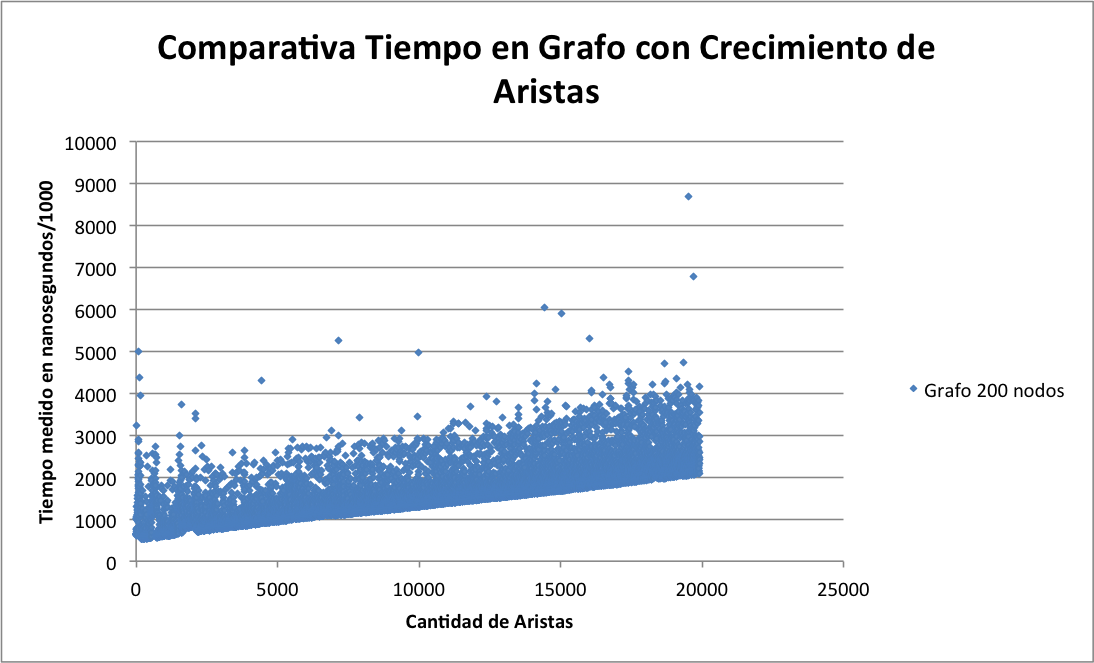
\includegraphics[width=140mm]{ejercicio1/ej1-grafo200-crecimientoaristas.png}
\centering 
\caption{Comparacion Tiempos de ejecucion - Cantiad de vertices fija, aristas variables}
\label{overflow3}
\end{figure}

Se puede ver que los tiempos aumentan linealmente a medida que la cantidad de aristas crece, esto se debe a que la creacion del grafo de predicados y la cantidad de elementos de las componentes conexas dependen fuertemente de N y M solo modifica la cantidad de conexiones que se crearan. \\

\pagebreak
\subsubsection{Analisis sobre N}

A continuaci\'on veamos que pasa cuando hacemos que M crezca de forma constante y aumentamos progresivamente N.\\
Los tiempos son en general mucho mayores y crecen m\'as r\'apido. Esto se debe nuevamente a que las operaciones sobre grafo de predicados y componentes conexas est\'an relacionadas con N y al aumentarlo, \'estas aumentan sus tiempos de ejecuci\'on. 

\begin{figure}[h!]
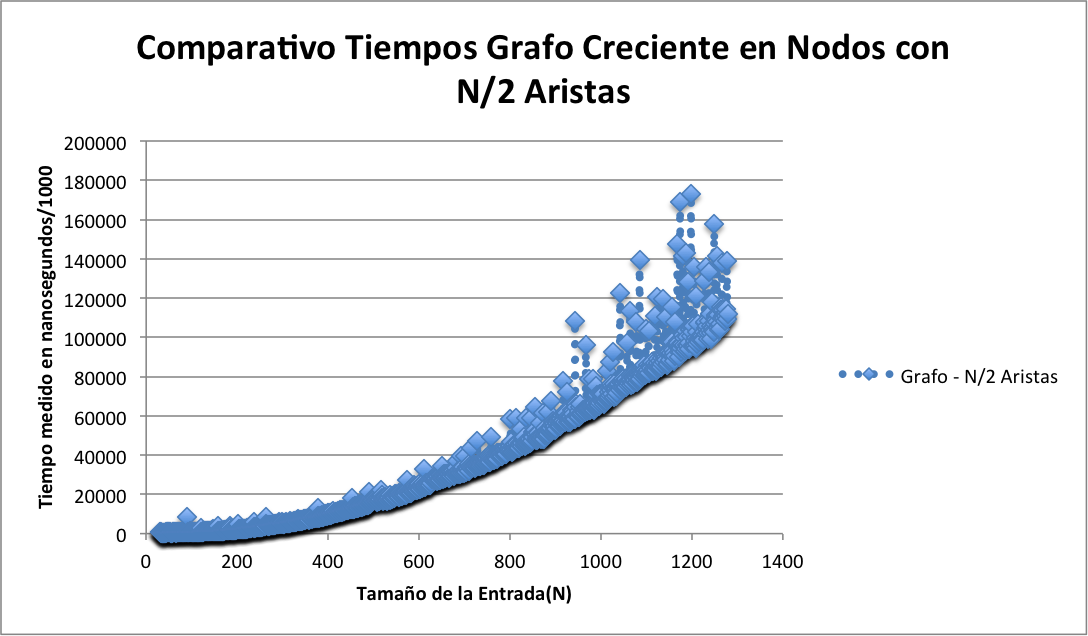
\includegraphics[width=140mm]{ejercicio1/ej1-grafo-nodosCreciente.png}
\centering
\caption{Comparacion Tiempos de ejecucion - Cantiad de aristas fija, nodos variables}
\label{overflow3}
\end{figure}

\pagebreak
\subsubsection{Analisis sobre Nodos y Colores}

Tuvimos la hip\'otesis de que un grafo de 50 nodos con 2 colores disponibles se iba a comportar igual que uno de 100 nodos con 1 color disponible. Asumimos que esto iba a ser as\'i por la cantidad de NodosPredicado que se crear\'ian en funci\'on de colores disponibles multiplicado por N, eso hubiera creado 200 NP en ambos grafos y los tiempos tendr\'ian que haberse parecido. Asumiamos que esto iba a ser una regla general.\\

Cuando hicimos el test nos dimos cuenta que est\'abamos equivocados en asumir que las conexiones iban a ser iguales en ambos grafos. Sin embargo llegamos a un gr\'afico que nos muestra el corportamiento lineal en ambas instancias.


\begin{figure}[h!]
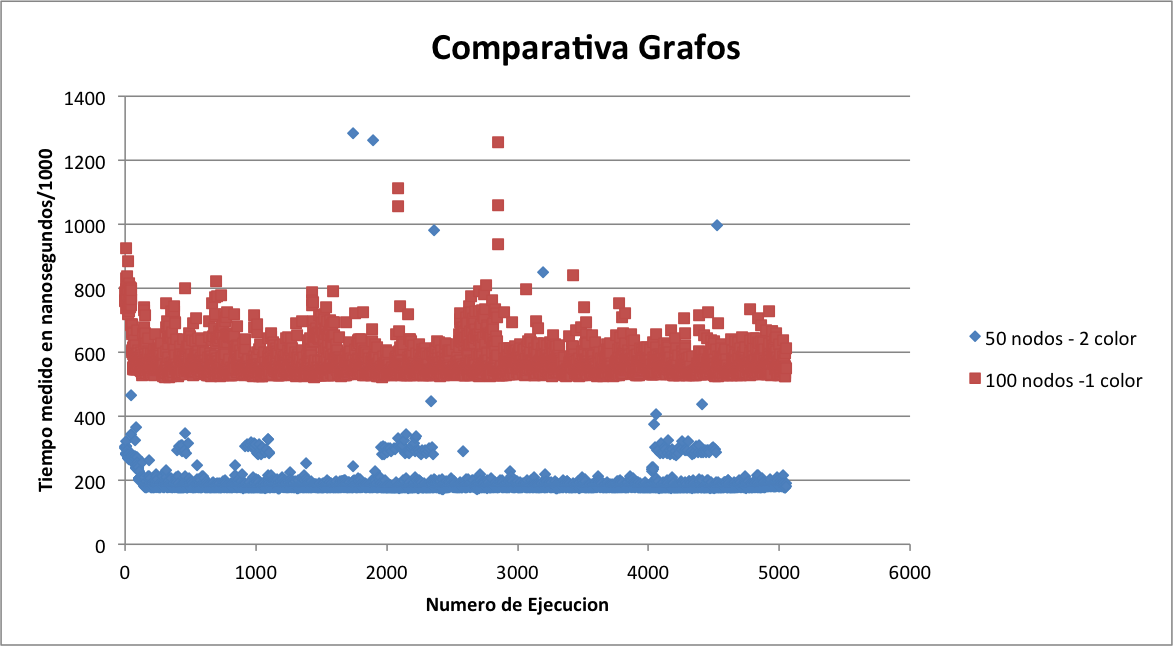
\includegraphics[width=140mm]{ejercicio1/ej1-grafo-relacionado.png}
\centering
\caption{Analisis sobre Nodos y Colores}
\label{overflow3}
\end{figure}

\pagebreak
\subsubsection{Generador de grafos}
Para generar nuestros grafos pseudo-aleatorios utilizamos el siguiente m\'etodo:\\
De antemano sabemos nuestros $N$ y $M$, tenemos un Array de nodos $[n_1,n_1,...,n_n]$,  comenzando desde $n_1$ buscamos el siguiente nodo $n_i$ con el que no tenga conexi\'on. Lanzamos una moneda cargada con una probabilidad, si da cara, conectamos el primer $n_1$ con nuestro $n_i$ y a $n_i$ con $n_1$. Repetimos hasta tener M conexiones o probar conectar $n_1$ con $n_n$, luego repetimos probando conexiones de $n_2$ y as\'i sucesivamente.

Los tiempos que figuran en el gr\'afico se deben a que al tener una probabilidad alta, las conexiones se hacen mucho m\'as rapido y esto trae como consecuencia que el grafo que se arma tenga componentes conexas m\'as grandes y que contienen nodos con id's m\'as bajas (Una alternativa para que las id's est\'en bien distribuidas era randomizar el orden de los nodos en el Arreglo, pero no lo tuvimos en cuenta).\\

Al variar la probabilidad vemos que con 75 se forman componentes m\'as pequenias y esto hace que el tiempo de  ejecuci\'on en grafos formados con esta probabilidad sea m\'as grande.

\begin{figure}[h!]
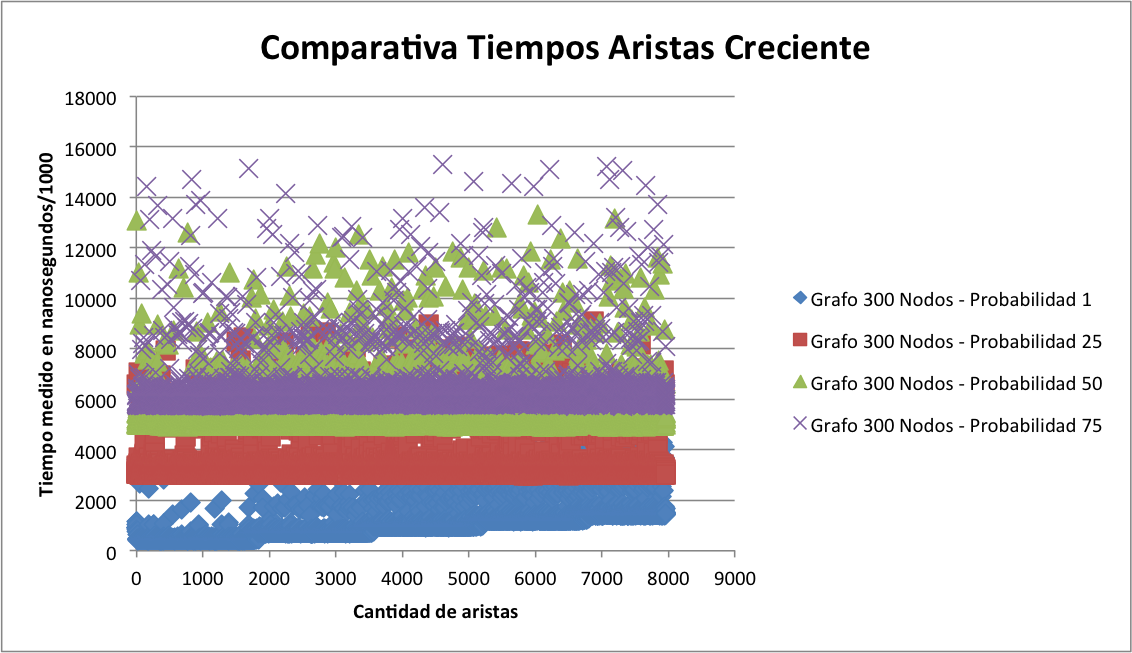
\includegraphics[width=140mm]{ejercicio1/ej1-grafo-aristasCreciente.png}
\centering
\caption{Tiempos de ejecuci\'on en grafos generados de distintas formas.}
\label{overflow3}
\end{figure}


\pagebreak